

\documentclass{article}
\usepackage[report, landscape]{geometry}
\geometry{
 a4paper,
 left=10mm,
 right=10mm,
 bottom=20mm,
 top=2mm,
 }
\usepackage{url}
\usepackage{multicol}
\usepackage{amsmath}
\usepackage{esint}
\usepackage{bigints}
\usepackage{amsfonts}
\usepackage{xcolor}
\usepackage{tikz}
\usetikzlibrary{calc}
\usetikzlibrary{decorations.pathmorphing}
\usepackage{amsmath,amssymb}
\usepackage{graphicx}
\graphicspath{ {./src/img/} }

\usepackage{colortbl}
\usepackage{xcolor}
\usepackage{mathtools}
\usepackage{amsmath,amssymb}
\usepackage{enumitem}
\usepackage{xhfill}
\makeatletter

\newcommand*\bigcdot{\mathpalette\bigcdot@{.5}}
\newcommand*\bigcdot@[2]{\mathbin{\vcenter{\hbox{\scalebox{#2}{$\m@th#1\bullet$}}}}}
\makeatother

\title{física eléctrica}
\usepackage[brazilian]{babel}
\usepackage[utf8]{inputenc}
\parindent0pt
\parskip2pt
\newcommand{\hr}{\centerline{\rule{3.5in}{1pt}}}
%\colorbox[HTML]{e4e4e4}{\makebox[\textwidth-2\fboxsep][l]{texto}
\newcommand{\nc}[2][]{%
\tikz \draw [draw=black, ultra thick, #1]
    ($(current page.center)-(0.5\linewidth,0)$) -- 
    ($(current page.center)+(0.5\linewidth,0)$)
    node [midway, fill=white] {#2};
}%
\begin{document}

\tikzstyle{mybox} = [draw=black, fill=white, very thick,
    rectangle, rounded corners, inner sep=10pt, inner ysep=10pt]
\tikzstyle{fancytitle} =[fill=black, text=white, font=\bfseries]

\newcommand{\nc}[2][]
{\tikz \draw [draw=black, ultra thick, #1]
($(current page.center)-(0.5\linewidth,0)$) -- 
($(current page.center)+(0.5\linewidth,0)$)
node [midway, fill=white] {#2};}

%---------------------------------
% \begin{tikzpicture}
% \node [mybox] (box){%
%     \begin{minipage}{0.33\textwidth}
% 	\nc{Biot-Savart}
% 	$d\vec{B}=\frac{\mu_o}{4\pi}\frac{Id\vec{l}\times\vec{r}}{r^3}$\\
% 	$B=\frac{\mu_oI}{4\pi R^2}\Delta l_{arco}$\\
% 	$B=\frac{\mu_oI}{4\pi R}(cos\theta_1-cos\theta_2)$\\
% 	\nc{Cargas en Movimiento}\\
% 	$r=\frac{mv}{qB}$\\
% 	$a=\frac{qvB}{m}=\frac{v^2}{r}$
% 	\end{minipage}
% };
%---------------------------------
% \node[fancytitle, right=10pt] at (box.north west) {Cargas en Movimiento con Presencia de Campos};
% \end{tikzpicture}
% \bigskip\\


\newcommand{\equationEntry}[2]
{
    \begin{minipage}{.29\textwidth}
        \vspace{.2in}
        \nc{#1}
        #2
    \end{minipage}
    \bigskip
}





\tikzstyle{mybox} = [draw=black, fill=white, very thick,
rounded corners, inner ysep=10pt, inner xsep=10pt]
\tikzstyle{fancytitle} =[fill=black, text=white, font=\bfseries]

\begin{document}

\begin{center}{\huge{\textbf{}}}\\
\end{center}
\begin{center}
    \begin{multicols}{3}
        \textbf{APRAKSTOŠĀ STATISTIKA}

\equationEntry{Vidējais aritmētiskais:}
{\begin{align*}
     \overline{x} &= \frac{\sum{i=1}{n}x_i}{0} \\
\end{align*}}

\equationEntry{Mediānas pozīcija:}
{\begin{align*}
    \frac{n+1}{2}
\end{align*}}

\equationEntry{Ģeometriskais vidējais:}
{\begin{align*}
    \sqrt[n]{x_1*x_2*\dots*x_n}
\end{align*}}

\equationEntry{Amplitūda (rangs):}
{\begin{align*}
    range(X)=X_{max}-X_{min}
\end{align*}}

\equationEntry{Dispersija (variance) izlasei:}
{\begin{align*}
    s^2 &= VARIANCE.S(X) \\
    s^2 &= \frac{\sum_{i=0}^{n} (x_i-\overline{x})^2}{n-1}
\end{align*}}

\equationEntry{Dispersija (variance) ģenerālkopai:}
{\begin{align*}
    \sigma^2 &= VARIANCE.P(X) \\
    \sigma^2 &= \frac{\sum_{i=0}^{n} (x_i-\overline{x})^2}{N}
\end{align*}}

\equationEntry{Standartnovirze (standartkļūda) izlasei:}
{\begin{align*}
    s &= STDEV.S(X) \\
    s &= \sqrt{s^2} \\
\end{align*}}

\equationEntry{Standartnovirze (standartkļūda) ģenerālkopai:}
{\begin{align*}
    s &= STDEV.P(X) \\
    \sigma &= \sqrt{\sigma^2}
\end{align*}}



\equationEntry{Standartizētā vērtība (Z-score):} 
{\begin{align*}
    Z &= \frac{x-\overline{x}}{s} \\
    Z &= \frac{x-\overline{x}}{\sigma}
\end{align*}}

\equationEntry{Asimetrijas koeficients:}
{

    \vspace*{.1in}
    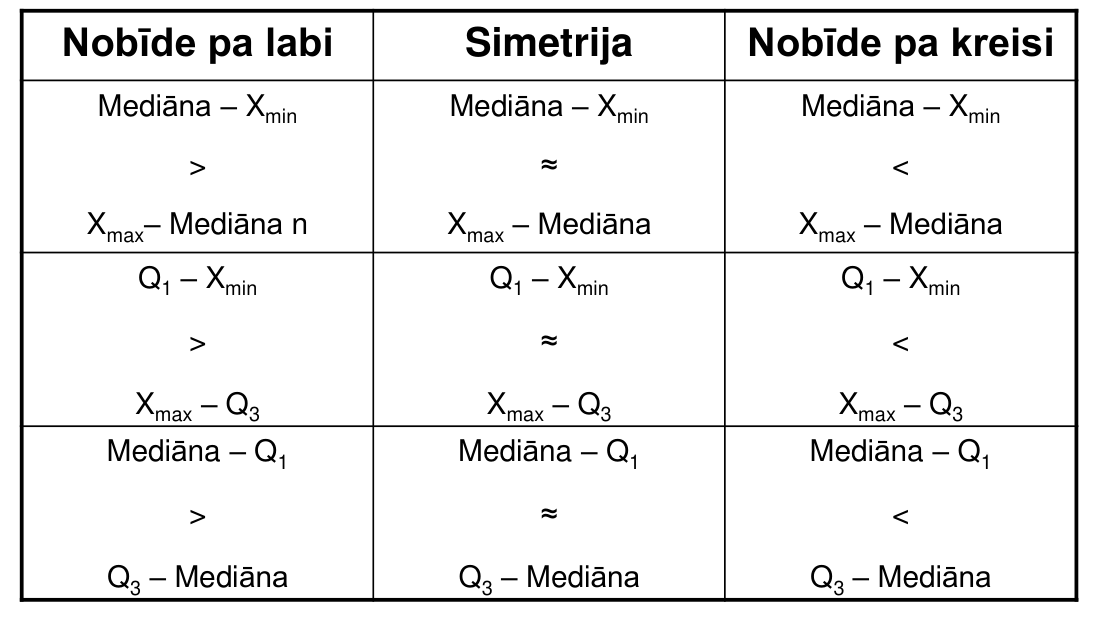
\includegraphics[width=1\textwidth]{SymmetryTable}
}

\equationEntry{Kvartiles:}

{

    If we have an ordered dataset $ x_{1},x_{2},...,x_{n}$, we can interpolate
    between data points to find the p pth empirical quantile if $x_{i}$ is in
    the ${\displaystyle i/(n+1)}$ quantile. If we denote the integer part of a
    number $a$ by $\lfloor a\rfloor$ , then the empirical quantile function is
    given by,

    \begin{align*}
        q(p/4) &= x_k + \alpha ( x_{k + 1} - x_k ) = QUARTILE.EXC(Arr, p) \\
        k &=\lfloor p(n+1)/4\rfloor \\
        \alpha &=p(n+1)/4-\lfloor p(n+1)/4\rfloor
    \end{align*}

    To find the first, second, and third quartiles of the dataset we would
    evaluate $q(0.25), q ( 0.5 ) q(0.5), and q ( 0.75 ) q(0.75)$ respectively. 

}

\equationEntry{Starpkvartiļu rangs (IQR):}
{
    \begin{align*}
        IQR &= Q_3-Q_1
    \end{align*}
}


\equationEntry{Kastes diagramma (Box plot)}
{
    \vspace*{.1in}
    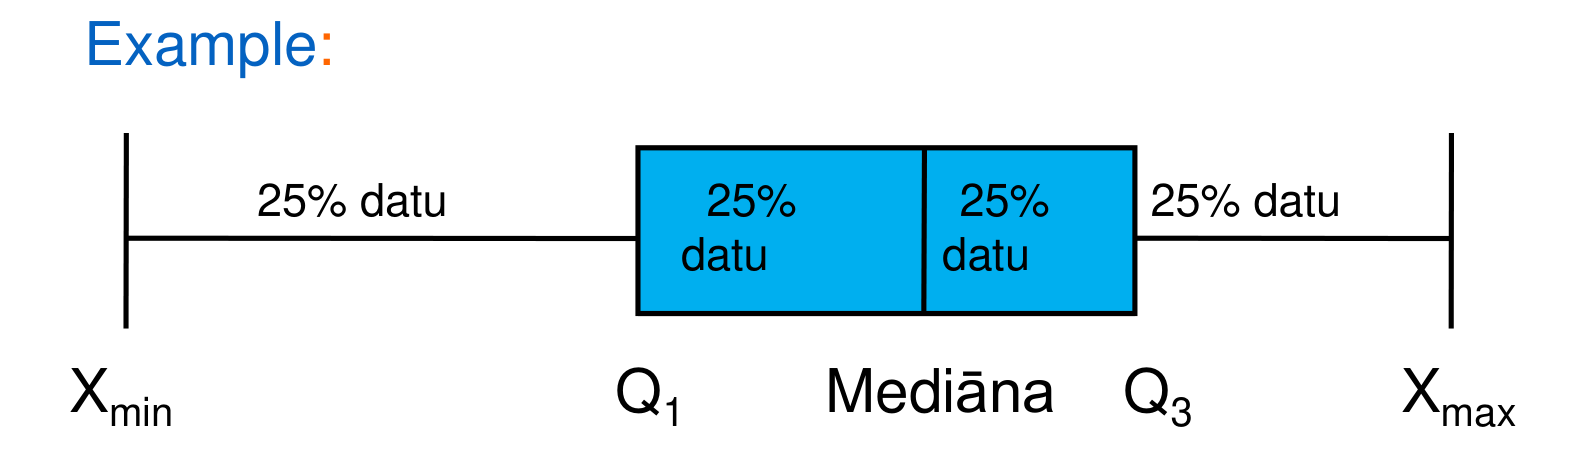
\includegraphics[width=1\textwidth]{BoxPlot}
}

\equationEntry{Kovariācijas koeficients}
{
    \begin{align*}
        cov(X,Y) = \frac{\sum_{i=0}^{n} (X_i-\overline{X})(Y_i-\overline{Y_i})}{n-1}
    \end{align*}
}

\linebreak
\textbf{Notikumi}

\equationEntry{Kombinācijas (secība nav svarīga):}
{\begin{align*}
    C_n^k &= (\frac{n}{k}) = \frac{n!}{k!(n-k)!} = COMBIN(n, k)
\end{align*}}

\equationEntry{Kombinācijas ar atkārojumiem (secība nav svarīga):}
{\begin{align*}
    TODO: excel
    \overline{C}_n^k &= COMBINA(n, k) \\
\end{align*}}

\equationEntry{Variācijas(secība ir svarīga):}
{\begin{align*}
    A_n^k = \frac{n!}{(n-k)!}
\end{align*}}

\equationEntry{Pretējais notikums:}
{\begin{align*}
    P(\lnot A ) = 1 - P (A)
\end{align*}}

\equationEntry{Neatkarīgo notikumu šķelums:}
{\begin{align*}
    P(A \land B) = P(A) * P(B)
\end{align*}}

\equationEntry{Neatkarīgo notikumu disjunkcija:}
{\begin{align*}
    P(A \lor B) = P(A) + P(B) - P(A \land B)
\end{align*}}

\equationEntry{Nesavienojamo notikumu disjunkcija:}
{\begin{align*}
    P(A \lor B) = P(A) + P(B)
\end{align*}}

\equationEntry{Nosacītā varbūtība:}

{

    $P(B|A)$ - B, ja zināms, ka A notika.
    \begin{align*}
        P(A|B) &= \displaystyle\frac{P(A \land B)}{P(B)} \\
        P(B|A) &= \displaystyle\frac{P(A \land B)}{P(A)}
    \end{align*}
}


\equationEntry{Nosacītā varbūtība (neatkarīgiem notikumiem):}

{

    $P(B|A)$ - B, ja zināms, ka A notika.
    \begin{align*}
        P(A|B) &= P(A) \\ 
        P(B|A) &= P(B) 
    \end{align*}
}


\equationEntry{Atkarīgo notikumu reizināšana:}

{

    $P(B|A)$ - B, ja zināms, ka A notika.
    \begin{align*}
        P(A) = P(A)P(B|A) \\
    \end{align*}
}


\equationEntry{Pilnā varbūtība}

{
   TODO 
}

\equationEntry{Beiesa teorēma}

{

    TODO 
}


\vspace*{.5in}
\textbf{GADĪJUMLIELUMI}

\equationEntry{Sagaidāmā vērtība:}
{\begin{align*}
    E[X] &= \mu = \sum_{i=1}^{N}x_iP(X=x_i) \\
\end{align*}}

\equationEntry{Dispersija:}
{\begin{align*}
    \sigma^2 &= \sum_{i=1}^{N}[x_i-E[X]]^2P(X=x_i) = E[x^2] - (E[X])^2 \\
\end{align*}}

\equationEntry{Standartnovirze:}
{\begin{align*}
    \sigma &= \sqrt{\sum_{i=1}^{N}[x_i-E[X]]^2P(X=x_i)} = \sqrt{E[x^2] - (E[X])^2} \\
\end{align*}}

\equationEntry{Kovariācija:}
{\begin{align*}
     &= \sum_{i=1}^{N}[x_i-E[X]][y_i-E[Y]]P(X=x_i, Y=y_i)
\end{align*}}

\equationEntry{Divu diskrēto gadījumlielumu summa}
{\begin{align*}
    E(X+Y) = E(X) + E(Y)
\end{align*}}

\equationEntry{Divu diskrēto gadījumlielumu dispersija}
{\begin{align*}
    Var(X+Y) = \sigma_{x+y}^2 = \sigma{x} + \sigma{y} + 2\sigma_{xy}\\
\end{align*}}

\equationEntry{Divu diskrēto gadījumlielumu standartnovirze}
{\begin{align*}
    \sigma_{x+y} = \sqrt{\sigma_{x+y}} 
\end{align*}}


\equationEntry{Portfeļa ienesīgums (vidējais svērtais ienesīgums)}
{\begin{align*}
    E(P)=wE(X)+(1-w)E(Y)\\
\end{align*}

Kur $w$ = aktīva X īpatsvars portfelī $(1 - w)$ = aktīva Y īpatsvars portfelī.
}

\equationEntry{Portfeļa risks (svērtā izkliede)}
{\begin{align*}
    \sigma_P=\sqrt{w^2\sigma^2+(1-w)^2\sigma_Y^2+2w(1-w)\sigma_{XY}}
\end{align*}

Kur $w$ = aktīva X īpatsvars portfelī $(1 - w)$ = aktīva Y īpatsvars portfelī.
}

\equationEntry{Binomiālais sadalījums}
{\begin{align*}
    P(X=x | n,p)=\displaystyle\frac{n!}{x!(n-x)!}(1-\p)^{1-x}p^x
\end{align*}

Kur $p$ - notikuma varbūtība, $X$ - diskrēts gadījumlielums, $n$ - notikumu
(izmēģinājumu) skaits.}


\equationEntry{Binomiālais sadalījuma raksturlielumi}
{\begin{align*}
    \mu = E(X) &= np \\
    \sigma^2 &= np(1-p) \\
    \sigma &= \sqrt{np(1-p)}
\end{align*}}


\equationEntry{Puasona sadalījums (binom. aproksimācija)}
{\begin{align*}
    P(X=x|\lambda) &= \displaystyle\frac{e^{-\lambda}\lambda^x}{x!} \\
    P(X=x|\lambda) &= POISSON.DIST(X, \mu, CUMM.) 
\end{align*}

Kur $x$ = notikuma iestāšanās skaits, $\lambda$ = sagaidāmais notikumu skaits
(Puasona sadalījuma vidējā vērtība), $\lambda$ = np, $e$ = naturālā logaritma
bāze ($2.71828...$ vai $EXP(1)$)
}
\equationEntry{Puasona sadalījuma raksturlielumi}
{\begin{align*}
    \mu &= \lambda \\
    \sigma^2 &= \lambda \\
    \sigma &= \sqrt{\lambda}
\end{align*}
}

\equationEntry{Ģeometriskais sadalījums (Hiperģeometriskais)}
{\begin{align*}
    P(X=x|n,N,E)=\displaystyle\frac{(\frac{E}{x})(\frac{N-E}{n-x})}{(\frac{N}{n})} \\
\end{align*}

    Kur $N$ = ģenerālkopas lielums, $E$ = interesējošo vienumu skaits
    ģenerālkopā, $n$ = izlases lielums, $x$ = interesējošo vienumu skaits
    izlasē.
}


\equationEntry{Ģeometriskais sadalījuma raksturlielumi}
{\begin{align*}
    E[x]&=\displaystyle\frac{nE}{N} \\
    \sigma &= \sqrt{\displaystyle\frac{nE(N-E)}{N^2}}*\sqrt{\displaystyle\frac{N-n}{N-1}}
\end{align*}}






\equationEntry{Eksponenciālais sadalījums}
{\begin{align*}
    f(X) &= EXPON.DIST(x, lambda, 0)\\
    f(X) &= \lambda e^{-\lambda X}, \> X > 0\\
    F(X) &= EXPON.DIST(x, lambda, 1)\\
    F(X) &= 1 -  e^{-\lambda X} \\
\end{align*}

Kur $\lambda$ - vidējais notikuma iestāšanas skaits laika vienībā.
}



\textbf{NORMĀLAIS SADALĪJUMS}

\equationEntry{Sadalījuma aprēkināšana:}
{\begin{align*}
    x = NORM.DIST(X, \mu, \sigma, CUMM) \\
\end{align*}}


\equationEntry{Vērtības un $\sigma$ iegūšana no varbūtības:}
{\begin{align*}
    Z &= NORM.S.INV(x) \\
    \sigma &= \displaystyle\frac{x-\mu}{Z} 
\end{align*}}





    \end{multicols}
\end{center}
\end{document}
